%\def \headmark {MODIFIED CONSTITUENTS IN IDIOM PROCESSING }
\documentclass[output=paper]{langsci/langscibook}

\markuptitle{\textit{Can you reach for the planets or grasp at the stars?} – 
Modified noun, verb, or preposition constituents in idiom processing}{Can you reach for the planets or grasp at the stars?}

\renewcommand*{\lsCollectionPaperFooterTitle}{{\noexpand\textit{Can you reach for the planets or grasp at the stars?} -- Modified noun, verb, or preposition constituents in idiom processing}}

\author{Eva Smolka\affiliation{University of Konstanz, Germany}\lastand Carsten Eulitz\affiliation{University of Konstanz, Germany}}

% \chapterDOI{} %will be filled in at production

% \epigram{}

\abstract{Idioms are a special case of multi-word expressions in that their meaning cannot be compositionally constructed from the meaning of the single constituents. The present study examines whether the figurative meaning of an idiom is recognized if critical idiomatic constituents (e.g. noun, verb, preposition) are modified. In three paraphrase experiments, participants saw (a) the canonical idiomatic phrase (e.g., \textit{She reached for the stars}), (b) the idiomatic phrase with a modified constituent (e.g., \textit{She reached/grasped for/at the stars/planets}), or (c) a matched literal control sentence (e.g., \textit{She reached for the sweets}) and rated how strongly the sentence reflected the meaning of a paraphrase of the idiom (e.g., \textit{She has always aspired to unattainable goals}).

Canonical idiomatic phrases and control sentences received highest and lowest paraphrase ratings, respectively, with modified constituents in between. Further, idioms with modified verbs were rated higher in matching the figurative meaning than idioms with modified prepositions or nouns. These findings indicate that the figurative meaning was assembled in spite of the modifications and support the notion that idioms are not fully 'semantically fixed’, but that modified constituents that activate meanings similar to those of the canonical constituents are good candidates in contributing to the figurative meaning of an idiom.  We discuss psycholinguistic models on idiom comprehension.} 

\begin{document}
\maketitle

\section{Introduction}   

Idioms like \textit{nach den Sternen greifen} (literal, L, and figurative, F, translation: ‘reach for the stars’) represent a special type of multiword expression. As with other semantically opaque word formations, the figurative meaning of idioms is not derived compositionally from the meaning of the constituents and their syntactic assembly. For example, the figurative meaning of the idiom \textit{She spilled the beans} cannot be derived by combining the meaning of the individual constituents (\textit{she, spilled, the, beans}) and their syntactic combination (‘an agent spilling some object’) as would be the case in \textit{She spilled the coffee}, despite the parallel syntactic structure. Hence, one of the aims of linguistic theory (e.g., \citealt{grice:1975,grice:1978}) has been the formulation of distinguishing criteria for idiomatic as compared to literal multiword expressions. The most important of these are semantic fixedness and syntactic anomaly. Semantic fixedness specifies that the figurative meaning does not allow the replacement of any of the constituents (e.g.\textit{*she dropped the beans; *she spilled the seeds/pellets}), while syntactic fixedness indicates that the figurative meaning restricts the syntactic transformations that an idiomatic expression may undergo (e.g.\textit{*the beans were spilled by her; *she spilled the secret beans}).


Linguistic and psycholinguistic researchers are thus baffled by the question of how idiomatic meaning is processed and stored in lexical memory (\citealt{burger:2003,burger:2004,cacciari:1994,gibbs:1994,gibbs:2002,swinney:1979}; for a review see \citealt{titone:1999,titone:2014}). In particular, it remains an unresolved question whether the meaning of an idiom is represented separately from the meaning of its parts, and how the figurative meaning is assembled. Seminal studies argued for a non-compositional representation in which the whole figurative meaning of an idiomatic phrase is stored as a distinct entry, the idiom word in the mental lexicon similar to the representation of a complex word like \textit{Finanzmarktaufsichtsbehörde} (‘financial market supervisory authority’). Idiomatic processing, the process by which figurative meaning is retrieved is thus assumed to be independent from the process by which literal meaning is computed \citep{bobrow:1973,gibbs:1980,swinney:1979}. 

In contrast, hybrid approaches assume that idioms are both unitary (i.e. each idiom possesses a distinct lexical entry for its figurative meaning) and compositional (i.e. composed of the single word lemmas of the constituents). The constituents are first processed literally until the idiom key or something akin to a unitary entry that carries the idiomatic concept is reached and activated \citep{cacciari:1988,caillies:2007,connine:1992,cutting:1997,gibbs:1989,holsinger:2013,sprenger:2006,titone:1999}. For example, even though idioms are syntactically analyzed similar to literal sentences, \citet{cutting:1997} postulate a distinct lexical concept node that is activated by the idiomatic concept. Similarly, \citet{sprenger:2006} assume a so-called superlemma like \textit{spill-the-beans} that specifies the information relating to that idiom, such as the single constituents (i.e. \textit{spill}, \textit{the}, and \textit{beans}), their syntactic functions (subject, direct object), syntactic categories (noun phrase, prepositional phrase), and parts of speech (noun, verb). Other hybrid models assume that the literal meanings of the constituents are activated only before the unitary entry is reached. For example, the configuration hypothesis (e.g., \citealt{cacciari:1988}) postulates a so-called idiom-key – the point at which the specific word configuration renders an idiom with figurative meaning. Words of a sentence are processed in a literal way until the idiom key is reached and the word formation is recognized as expressing figurative meaning. As soon as the idiom key has been hit, only the figurative meaning of the idiom is processed and remains activated, while the literal activations disappear. 

However, Smolka and colleagues \citep{rabanus:2008,smolka:2007} observed that the literal meaning of verbs remains accessible even after the idiom key has been hit. In two sentence priming experiments, participants read an idiomatic sentence, such as \textit{Sie hat ihm gründlich den Kopf gewaschen} (word by word, W: ‘she has him thoroughly the head washed’; literal, L: ‘She thoroughly washed his head’; figurative, F: `She gave him a piece of her mind') and made lexical decisions about words associated with the figurative meaning (e.g. \textit{Standpauke} ‘telling-off’), about associations with the literal meaning of the verb (e.g. \textit{Kleidung} ‘clothes’), and about matched unrelated words. 

Because all sentences were highly predictable (i.e., with cloze probabilities, on average, higher than 87\%), the idiom key -- the point at which the constituents are recognized to form an idiom -- should occur before the sentence-final word (e.g. \textit{gewaschen} ‘washed’). The sentences were presented visually and targets were presented 500\,ms after the presentation of the verb participle to make sure that the figurative meaning was available. Under these experimental conditions, the configuration hypothesis \citep{cacciari:1988} predicts figurative meaning activations only. However, the results of both studies showed that associations with the literal meaning of the verb were activated to the same degree as were associations with the figurative meaning.  

The authors concluded that (1) the literal meaning of single word constituents is accessed during figurative processing and that (2) the literal meaning, at least that of verbs, remains activated even after the figurative meaning of the idiom has been recognized (e.g., \citealt{cacciari:1988}; \citealt{cutting:1997}; \citealt{sprenger:2006}). Note that hybrid models, assuming an idiom key, specify that the literal meaning of the constituents is not recalled as soon as the figurative meaning of the idiom is recognized, and (3) described a model on idiom comprehension that incorporates the complexity of idiom processing: the meaning of the single constituents is activated, and the joint co-activation of the single constituents activates the figurative meaning at the conceptual level.

The above findings give rise to the following questions: if a single idiomatic constituent activates its literal meaning alongside the figurative meaning, and if the joint activation of idiomatic constituents triggers the figurative meaning, will a close associate of the idiomatic constituent (that activates a similar meaning) contribute to the activation of the figurative meaning of the idiom? For example, will the word \textit{planets} in the configuration \textit{reach for the planets} activate the figurative meaning of \textit{reach for the stars}? A positive finding would indicate that idioms are not as semantically fixed as current models on idiom processing assume (e.g., \citealt{sprenger:2006}). Furthermore, are some constituents of the idiom more susceptible to modification than others? That is, does the word category of an idiomatic constituent -- whether it is a verb, a noun, or a preposition -- influence whether the constituent can be modified without losing the figurative meaning?

Indeed, in a recent study, \citet{geeraert:2017} observed that noun constituents of idioms may be modified to some degree. Participants rated the acceptability of idioms in their canonical form (e.g. \textit{...~they went through the ceiling}), when idioms were partial forms (e.g. \textit{...~they went through it}), when they held an integrated concept (e.g. \textit{...~they went through the investment roof}), or when they were idiom blends (e.g. \textit{...~they suddenly went through the charts}). Modifications of the idiom made it less acceptable, however, the degree of the acceptability depended on the type of the variation, indicating that modifications with near synonyms (\textit{roof – ceiling}) or integrated concepts (\textit{investment roof}) were more acceptable than other variations. The authors concluded that their findings challenge any theories on idiom processing that assume fixed units for the specification of the figurative meaning, be it multiword form units \citep{bobrow:1973}, superlemmas (e.g. \citealt{sprenger:2006}), or word configurations \citep{cacciari:1988}. 

The aim of the present study was to examine the semantic fixedness of idioms in more detail: (a) Will the figurative meaning of an idiom be retained, if an idiomatic constituent, such as the noun, verb, or preposition, is modified?  (b) Will the word category of an idiomatic constituent (noun, verb, preposition) affect whether a modification will preserve the figurative meaning?

For this purpose, we conducted three sentence paraphrase experiments. Each canonical idiomatic sentence, such as \textit{Sie hat immer nach den Sternen gegriffen} (L: ‘She always reached for the stars’; F: `She always reached for the stars’) was presented in three versions: (1) with its canonical constituent, (2) with the canonical constituent replaced by a closely associated word, or (3) with the canonical constituent replaced by an unrelated word. We manipulated the noun constituent in Experiment 1, the verb constituent in Experiment 2, and the preposition in Experiment 3. The idiomatic noun constituent (e.g. \textit{stars}) was replaced by a closely associated noun (e.g. \textit{planets}), as in \textit{Sie hat nach den Planeten gegriffen} (L: ‘She reached for the planets’) or by an unrelated noun (e.g. \textit{sweets}), as in \textit{Sie hat nach den Bonbons gegriffen} (L: ‘She reached for the sweets’). In Experiment 2, the idiomatic verb constituent (e.g. \textit{reach}) was substituted by a closely associated verb (e.g. \textit{grasp}), as in \textit{Sie hat nach den Sternen gelangt} (L: ‘She grasped at the stars’) or by an unrelated verb (e.g. \textit{ask}), as in \textit{Sie hat nach den Sternen gefragt} (L: ‘She asked for the stars’). In Experiment 3, the idiomatic preposition was replaced by another preposition, as in \textit{Sie hat zu den Sternen gegriffen} (L: ‘She reached to the stars’) or by an unrelated prepositional phrase (that held the original preposition of the idiom), as in \textit{Sie hat nach den Bonbons gegriffen} (L: ‘She reached for the sweets’).  Each sentence was paired with the paraphrase of the idiomatic sentence, \textit{Sie hat immer etwas Unerreichbares angestrebt} (L: ‘She always strived for something unreachable’), and participants rated on a scale from 1 to 7 how well the meanings of two sentences mirrored each other. Examples of idiomatic sentences, their modifications and paraphrases are given in Tables~\ref{tab:tripletsNouns}--\ref{tab:tripletsPrepositions}.

\begin{sidewaystable}\footnotesize
\caption{Examples of sentence triplets for idiomatic phrases with modified nouns and corresponding paraphrase. \textit{Notes:} W = word by word; L = literal; F = figurative\label{tab:tripletsNouns}}
% \resizebox{\textwidth}{!}{
\begin{tabularx}{\textwidth}{l@{\hspace{.5em}}l@{\hspace{.5em}}Ql@{\hspace{.5em}}l@{\hspace{.5em}}Q}
\lsptoprule
\multicolumn{3}{c}{Idiomatic/Modified/Unrelated}            & \multicolumn{3}{c}{Paraphrase}                                                     \\ \midrule
\multicolumn{3}{l}{\textit{Sie hat immer nach den Sternen/Planeten/Bonbons gegriffen.}}    & \multicolumn{3}{l}{\textit{Sie hat immer etwas Unerreichbares angestrebt.}}\\
& (W) & She has always for the stars/planets/sweets reached.               & & (W) & She has always something unreachable aspired.                                            \\
& (L) & She always reached for the stars/planets/sweets.                   & & (L) & She always aspired to something unreachable.                                             \\
& (F) & She always reached for the stars.                                  &                                                                                              \\ \tablevspace
\multicolumn{3}{l}{\textit{Sie haben die Katze im Sack/Beutel/Frühling gekauft.}}& \multicolumn{3}{l}{\textit{Sie wurden beim ungeprüften Kauf übervorteilt.}}\\
& (W) & They have the cat in the sack/bag/spring bought.                   & & (W) & They were at the uninspected purchase outsmarted.                                        \\
& (L) & They bought the cat in the sack/bag/spring.                        & & (L) & They were outsmarted at the uninspected purchase.                                        \\
& (F) & They bought a pig in a poke.                                       &                                                                                              \\ \tablevspace
\multicolumn{3}{l}{\textit{Sie hat immer aufs falsche Pferd/Ross/Spielfeld gesetzt.}}  & \multicolumn{3}{l}{\textit{Sie hat die Lage immer falsch eingeschätzt und sich}}  \\
\multicolumn{3}{l}{}                                                                   & \multicolumn{3}{l}{\textit{entsprechend falsch verhalten.}}\\
& (W) & She has always on the wrong horse/steed/playing field bet.         & & (W) & She has the position always wrongly evaluated and herself accordingly wrongly conducted. \\
& (L) & She always bet on the wrong horse/steed/playing field.             & & (L) & She always misgauged the situation and thus acted improperly.                            \\
& (F) & She always bet on the wrong horse.                                 &                                                                                              \\ \tablevspace
\multicolumn{3}{l}{\textit{Er hat sich mit fremden Federn/Daunen/Edelsteinen geschmückt.}} & \multicolumn{3}{l}{\textit{Er hat die Verdienste anderer als die eigenen ausgegeben.}}\\
& (W) & He has himself with foreign feathers/down/gemstones adorned.       & & (W) & He has the merits of others passed as the own ones. \\
& (L) & He adorned himself with foreign feathers/down/gemstones.           & & (L) & He passed off the merits of others as his own.   \\
& (F) & He adorned himself with borrowed plumes.                           &     \\ \lspbottomrule
\end{tabularx}
\end{sidewaystable}

\begin{sidewaystable}\footnotesize
\caption{Examples of sentence triplets for idiomatic phrases with modified verbs and their corresponding paraphrase. \textit{Notes:} W = word by word; L = literal; F = figurative\label{tab:tripletsVerbs}}
% \resizebox{\textwidth}{!}{
\begin{tabularx}{\textwidth}{l@{\hspace{.5em}}l@{\hspace{.5em}}Ql@{\hspace{.5em}}l@{\hspace{.5em}}Q}
\lsptoprule
\multicolumn{3}{c}{Idiomatic/Modified/Unrelated}                     & \multicolumn{3}{c}{Paraphrase}                                      \\ \midrule
\multicolumn{3}{l}{\textit{Sie hat immer nach den Sternen gegriffen/gelangt/gefragt.}}             & \multicolumn{3}{l}{\textit{Sie hat immer etwas Unerreichbares angestrebt.}}                      \\
& (W) & She has always for the stars reached/grasped/asked.                         & & (W) & She has always something unreachable aspired.                             \\ 
& (L) & She always reached for/grasped at\slash asked for the stars.                & & (L) & She always aspired something unreachable.                                 \\
& (F) & She always reached for the stars.                                           &                                                                               \\ \tablevspace
\multicolumn{3}{l}{\textit{Mir ist ein Stein vom Herzen gefallen/gestürzt\slash vom Dach gerollt.}}     & \multicolumn{3}{l}{\textit{Ich bin darüber sehr erleichtert gewesen.}}                           \\
& (W) & To me is a stone from heart fallen/dropped\slash from the roof rolled.           & & (W) & I have about that very relieved been.                                     \\
& (L) & A stone fell/dropped off the heart\slash rolled off the roof.                    & & (L) & I was very relieved about that.                                           \\
& (F) & It took a load off my mind.                                                 &                                                                               \\ \tablevspace
\multicolumn{3}{l}{\textit{Er hat mir wieder einen Korb gegeben/gereicht/geflochten.}}              & \multicolumn{3}{l}{\textit{Er hat mich wieder abgewiesen.}}                                       \\
& (W) & He has me again a basket given/handed/woven.                                & & (W) & He has me again rejected.                                                 \\
& (L) & He again gave/handed/wove me a basket.                                      & & (L) & He rejected me again.                                                     \\
& (F) & He turned me down again.                                                    &                                                                               \\ \tablevspace
\multicolumn{3}{l}{\textit{Seine Frau hat ihm die Schau gestohlen/geklaut/}} & \multicolumn{3}{l}{\textit{Seine Frau ist an seiner Stelle zum Interessensmittelpunkt geworden.}} \\
\multicolumn{3}{l}{\textit{(die Hemden gebügelt).}}\\
& (W) & His wife has him the show stolen/lifted\slash (his shirts ironed).               & & (W) & His wife is on his place to the focus of attention become.                  \\
& (L) & His wife stole/lifted his show\slash (ironed his shirts).                        & & (L) & His wife occupied center-stage instead of him.                             \\
& (F) & His wife upstaged him.                                                      &                                                                               \\ \lspbottomrule
\end{tabularx}
% }
\end{sidewaystable}

\begin{sidewaystable}\footnotesize
\caption{Examples of sentence triplets for idiomatic phrases with modified prepositions and their corresponding paraphrase. \textit{Notes:} W = word by word; L = literal; F = figurative\label{tab:tripletsPrepositions}}
% \resizebox{\textwidth}{!}{
\begin{tabularx}{\textwidth}{l@{\hspace{.5em}}l@{\hspace{.5em}}Ql@{\hspace{.5em}}l@{\hspace{.5em}}Q}
\lsptoprule
\multicolumn{3}{C}{Idiomatic/Modified/(Unrelated Prepositional Phrase)}                 & \multicolumn{3}{c}{Paraphrase}      \\ \midrule
\multicolumn{3}{l}{\textit{Sie hat immer nach/zu den Sternen\slash (nach den Bonbons) gegriffen.}}          & \multicolumn{3}{l}{\textit{Sie hat immer etwas Unerreichbares angestrebt.}}           \\
& (W) & She has always for/at the stars/(for the sweets) reached.               & & (W) & She has always something unreachable aspired.    \\
& (L) & She always reached for/to the stars/(for the sweets).                   & & (L) & She always aspired something unreachable.    \\
& (F) & She always reached for the stars.                                       &                                                                   \\ \tablevspace
\multicolumn{3}{l}{\textit{Ich habe ihn sehr ins/ans Herz\slash (ins Zimmer) geschlossen.}}                & \multicolumn{3}{l}{\textit{Ich habe ihn sehr lieb gewonnen.}}\\
& (W) & I have him very into/at the heart\slash (into the room) locked.         & & (W) & I have him very dear won.                           \\
& (L) & I locked him into/at the heart\slash (into the room).                   & & (L) & I like him very much.      \\
& (F) & I have grown very fond of him.                                          &                                                                   \\ \tablevspace
\multicolumn{3}{l}{\textit{Sie sind auf/an keinen grünen Zweig/(auf keinen grünen Golfplatz)}} & \multicolumn{3}{l}{\textit{Trotz starker Bemühungen konnten sie sich nicht einigen.}} \\
\multicolumn{3}{l}{\textit{gekommen.}}\\ 
& (W) & They have on/at no green branch\slash (on no green golf course) come.   & & (W) & In spite of all efforts could they themselves not agree.  \\
& (L) & They didn’t arrive on/at a green branch\slash golf course.              & & (L) & Despite all efforts, they did not come to an understanding. \\
& (F) & They could not come to terms.                                           &                                                                   \\ \tablevspace
\multicolumn{3}{l}{\textit{Damit hat er Öl ins/aufs Feuer\slash (in den Tank) gegossen.}}                    & \multicolumn{3}{l}{\textit{Damit hat er den Streit und die Erregung noch verstärkt.}} \\
& (W) & Thereby has he oil into/onto\slash (into the tank) poured.                & & (W) & Thereby has he the dispute and the arousal even reinforced. \\
& (L) & By that he poured oil into/onto the fire\slash (into the tank).           & & (L) & By that he enforced the fight and the arousal even more.    \\
& (F) & By that he added fuel to the fire.                                       &                                                                   \\ \lspbottomrule
\end{tabularx}
\end{sidewaystable}

In all three experiments, we used idiomatic sentences and minimized the influence of some confounding variables by controlling the following factors: (a) the number of words in a sentence was alike, that is, each sentence was comprised of seven words; (b) all sentences had the same structure (subject-verb-prepositional phrase-participle) and all were presented in the perfect tense, so that the position of the verb was always sentence-final, and (c) all sentences had a high cloze probability (on average 90\%), ensuring that the sentence-final word was highly predictable. It was thus established that the phrasal meaning was processed and the word configuration was rendered as figurative before the last word of a sentence. Finally, to provide a strong basis for the generalization of our findings, we examined between 33 and 39 different idiomatic phrases in each experiment. 


If ``unitary'' entries define the idiomatic constituents, then sentences whose idiomatic constituents are replaced by close associates will not be considered to hold the figurative meaning and should yield paraphrase ratings similar to sentences with unrelated constituents. If, however, the assumptions hold (a) that each idiomatic constituent activates its literal meaning, (b) that a close associate of an idiomatic constituent will activate a similar literal meaning and (c) will thus contribute to the joint co-activation of the figurative meaning, sentences holding close associates of an idiomatic constituent will be rated as higher in reflecting the figurative meaning than those with unrelated constituents. Furthermore, if the assumption holds that the verb is the structural center of the phrase (as assumed by \citealt{rabanus:2008} and \citealt{smolka:2007}, the modification of the verb constituent will differ from that of the noun or preposition constituents. 

\section{Experiment 1}

\subsection{Method}
\subsubsection{Participants}
Thirty-six university students, all native speakers of German, participated in the experiment for course credit or payment.

\subsubsection{Materials}
Thirty-nine idiomatic phrases were selected for the sentence paraphrase test. We defined an idiomatic phrase as a verb phrase (a) where both the verb and its complement are used in a nonliteral way to produce an overall idiomatic interpretation, (b) that shows some kind of morphosyntactic anomaly, and (c) whose figurative meaning is lexicalized.  In the light of these three properties, the idiomaticity of the phrases selected was agreed upon by three independent judges and further verified by reference to an idiomatic phrase dictionary \citep{redewendungen:2002}.

Each idiomatic sentence consisted of seven words and was phrased in the perfect tense, rendering the past participle form of a verb in sentence-final position. All idiomatic sentences were chosen from the pool of sentences tested in the sentence-completion experiment described in \citet{smolka:2007}. To assure that their figurative meaning was the dominant reading, only idiomatic phrases with high sentence completion rates were selected. That is, these sentences were completed with words that produced the figurative meaning in 93\% of the cases (range 52\% to 100\%).

\subsubsubsection{Sentence completion task}
More than 1,100 sentences in literal and figurative meaning were tested in a sentence completion task (for a more detailed description see \citealt{smolka:2007}). For the completion task, the last word of a sentence (i.e. the past participle) was omitted and completed by between 25 and 32 monolingual native speakers of German in an online portal (\textit{Language experiments portal} by \citealt{keller:1998}). For each sentence, the number of sentence completions with a specific verb was counted. For example, 19 of the 25 participants who saw the sentence \textit{Sie hat immer nach den Sternen \noindent\rule{1cm}{0.4pt}} (L: `She always \noindent\rule{1cm}{0.4pt} for the stars') completed it with the participle \textit{gegriffen} (‘reached’) and thus finalized the sentence in its figurative meaning \textit{She always reached for the stars}. The other 6 participants completed the sentence with the verb \textit{geschaut} (‘looked at’) and thus yielded the literal meaning `She always looked at the stars'.

\subsubsubsection{Noun association test}  Each idiomatic sentence, such as \textit{She reached for the stars}, was phrased in three versions, holding either (a) the canonical idiomatic noun constituent (I), such as \textit{Sterne} (‘stars’), (b) an associated noun (A), such as \textit{Planeten} (‘planets’), or (c) an unrelated noun (U), such as \textit{Bonbons} (‘sweets’). Tables~\ref{tab:tripletsNouns}--\ref{tab:tripletsPrepositions} provides examples of idiomatic sentences and the noun modifications; \tabref{tab:stimulus} provide the stimulus characteristics of the idiomatic sentences and their corresponding noun constituents. 


\begin{table}
\caption{Idiomatic sentences and stimulus characteristics of the idiomatic, modified, and unrelated noun constituents in Experiment 1. \textit{Notes:} N = number of items, Lemma = mean lemma frequency per one million, taken from CELEX \citep{baayen:1993}, Closure = mean sentence completion in \%.\label{tab:stimulus}}
\resizebox{\textwidth}{!}{\begin{tabular}{ccSSS}
\lsptoprule
 &  & \multicolumn{3}{c}{Type of noun} \\ \cmidrule(lr){3-5}
 & {Idiomatic phrase} & {Idiomatic} & {Modified} & {Unrelated} \\ \midrule
Example       & \textit{Sie hat nach den Sternen gegriffen} & \textit{Sternen} & \textit{Planeten} & \textit{Bonbons}\\ 
(translation) & (L: ‘She reached for the stars')             & {(‘stars')} & {(‘planets')} & {(‘sweets')}\\ 
{N} &  & 39 & 39 & 39 \\ 
{Lemma} &  & 57.1 & 25.5 & 39.6 \\ 
{Surface} &  & 32.3 & 16.8 & 22.9 \\ 
{Association} &  & {--} & 5.8 & {--} \\ 
{Closure} &  & 93.1 & {--} & {--} \\ 
\lspbottomrule
\end{tabular}}
\end{table}


To find close associates, two noun associations (e.g. \textit{planets} and \textit{moons}) were selected for each of the idiomatic noun constituents that should be modified (e.g. \textit{stars} in the idiomatic phrase \textit{She reached for the stars}). Care was taken that the associations were unrelated with the figurative phrasal meaning, and that the gender and the number inflections of the noun associations fitted the original idiomatic sentence. To avoid episodic effects, the same noun occurred only once in the whole experiment.

The strength of the associations was assessed in a pre-test that comprised two lists. The two noun associates of the idiomatic constituents were allocated to two lists; in both lists, the idiomatic noun constituent was paired with its associated noun and with an unrelated noun.  For example, in List 1, the idiomatic constituent \textit{Sterne} (‘stars’) was presented with the association \textit{Planeten} (‘planets’) and the unrelated noun \textit{Praxis} (‘practice’); in List 2, \textit{Sterne} (‘stars’) was presented with \textit{Monde} (‘moons’) and \textit{Praxis} (‘practice’).

Forty participants (who did not participate in the paraphrase experiment) rated on a scale from 1 (not at all) to 7 (strongly) how strongly the two nouns (e.g., \textit{stars – planets}) are meaning-related. Noun associations were selected as modifications of the original idiomatic noun, if they received high ratings (mean rating 5.8), and if their lemma and surface frequencies (taken from CELEX, see \citealt{baayen:1993}) were well matched with those of the idiomatic constituent. 

\subsubsubsection{Paraphrases} 
For each idiomatic phrase, we constructed a paraphrase by looking up the definition of the idiom in the idiomatic phrase dictionary \citep{redewendungen:2002}. For a similar appearance as the idiomatic sentence, the paraphrase was cast in the past perfect tense and with the same subject as that of the idiomatic phrase. 

\subsubsection{Procedure}
Three lists were constructed, each included one of the sentence triplets of an idiomatic phrase.  The three versions of an idiomatic phrase were rotated over the three lists by Latin square in such a way that a list contained the idiomatic sentence either with the canonical idiomatic (I), the associated (A), or the unrelated (U) noun. Each of the three sentence triplets was paired with the same paraphrase of the idiomatic sentence (see \tabref{tab:tripletsNouns} for examples). Altogether, each list comprised 39 sentence pairs. 

Each participant saw only one of the three lists, assignment to lists was randomized. Paraphrase tests were distributed via email. Participants were asked to rate (on a scale from 1 to 7) how strongly the two sentences reflected each other’s meaning. The instructions included two examples: one sentence pair with high meaning relatedness, the other sentence pair with low meaning relatedness. 

\subsection{Results}

In this and the following experiments, we used R \citep{rCore:2012} and lme4 (e.g., \citealt{bates:2005}; \citealt{bates:2012}; \citealt{baayen:2008}) to perform linear mixed effects modeling (LMM). As random effects, we had intercepts for participants and items (i.e. sentences). As fixed effects, we included the factor Modification Type (idiomatic/associated/unrelated), the Sentence Closure of the idiomatic phrase, and the Frequency of the constituent. The absolute and normalized lemma frequencies were taken from the CELEX lexical database \citep{baayen:1993} and were log-transformed and centered (e.g. \citealt{winter:2013}). All \textit{p}-values were calculated on the basis of Satterthwaite approximation by using the \texttt{lmerTest} package \citep{kuznetsova:2015}. In this and the following experiments, we applied a forward procedure for the model selection, starting with a minimal model and adding additional predictors only when they improved the model fit. The best model fit was obtained by comparing the Akaike Information Criterion (AIC) statistics between models, with a difference between models $>4$ \citep{sakamoto:1986}. 

\begin{table}
\caption{Fixed effects of the predictors in the linear mixed-effect model for the paraphrase ratings in Experiment 1. \textit{Notes:} significance code: *** < 0.0001.\label{tab:linear}}
\resizebox{\textwidth}{!}{\begin{tabular}{lS[table-format=-1.3]S[table-format=1.3]S[table-format=3.1]SS[table-format=<1.2e2]l}
\lsptoprule
 & {Estimate} & {Std. Error} & {df} & {$t$-value} & {$p$} &  \\ \midrule
(Intercept: Idiomatic) & 6.246 & 0.179 & 123.1 & 34.83 & <2.00e-16 & *** \\ 
Constituent (Modified) & -2.115 & 0.210 & 112.8 & -10.08 & <2.00e-16 & *** \\ 
Constituent (Unrelated) & -3.722 & 0.210 & 112.8 & -17.73 & <2.00e-16 & *** \\
\lspbottomrule
\end{tabular}}
\end{table}


The LMM analysis of Experiment 1 indicated that the best model fit included the fixed-effect factor Modification Type, no other fixed-effect factors were significant.  \tabref{tab:linear} summarizes the effects; the left panel of \figref{fig:chart} depicts the ratings. Results were straightforward: Paraphrase ratings were highest to idiomatic phrases that held the canonical idiomatic noun constituent (mean = 6.25, SD = 1.81), lower to phrases in which the canonical noun was modified by a closely associated noun (mean = 4.13, SD = 2.33), and lowest to phrases with unrelated nouns (mean = 2.52, SD = 2.21).

\begin{figure}[hbt!]
  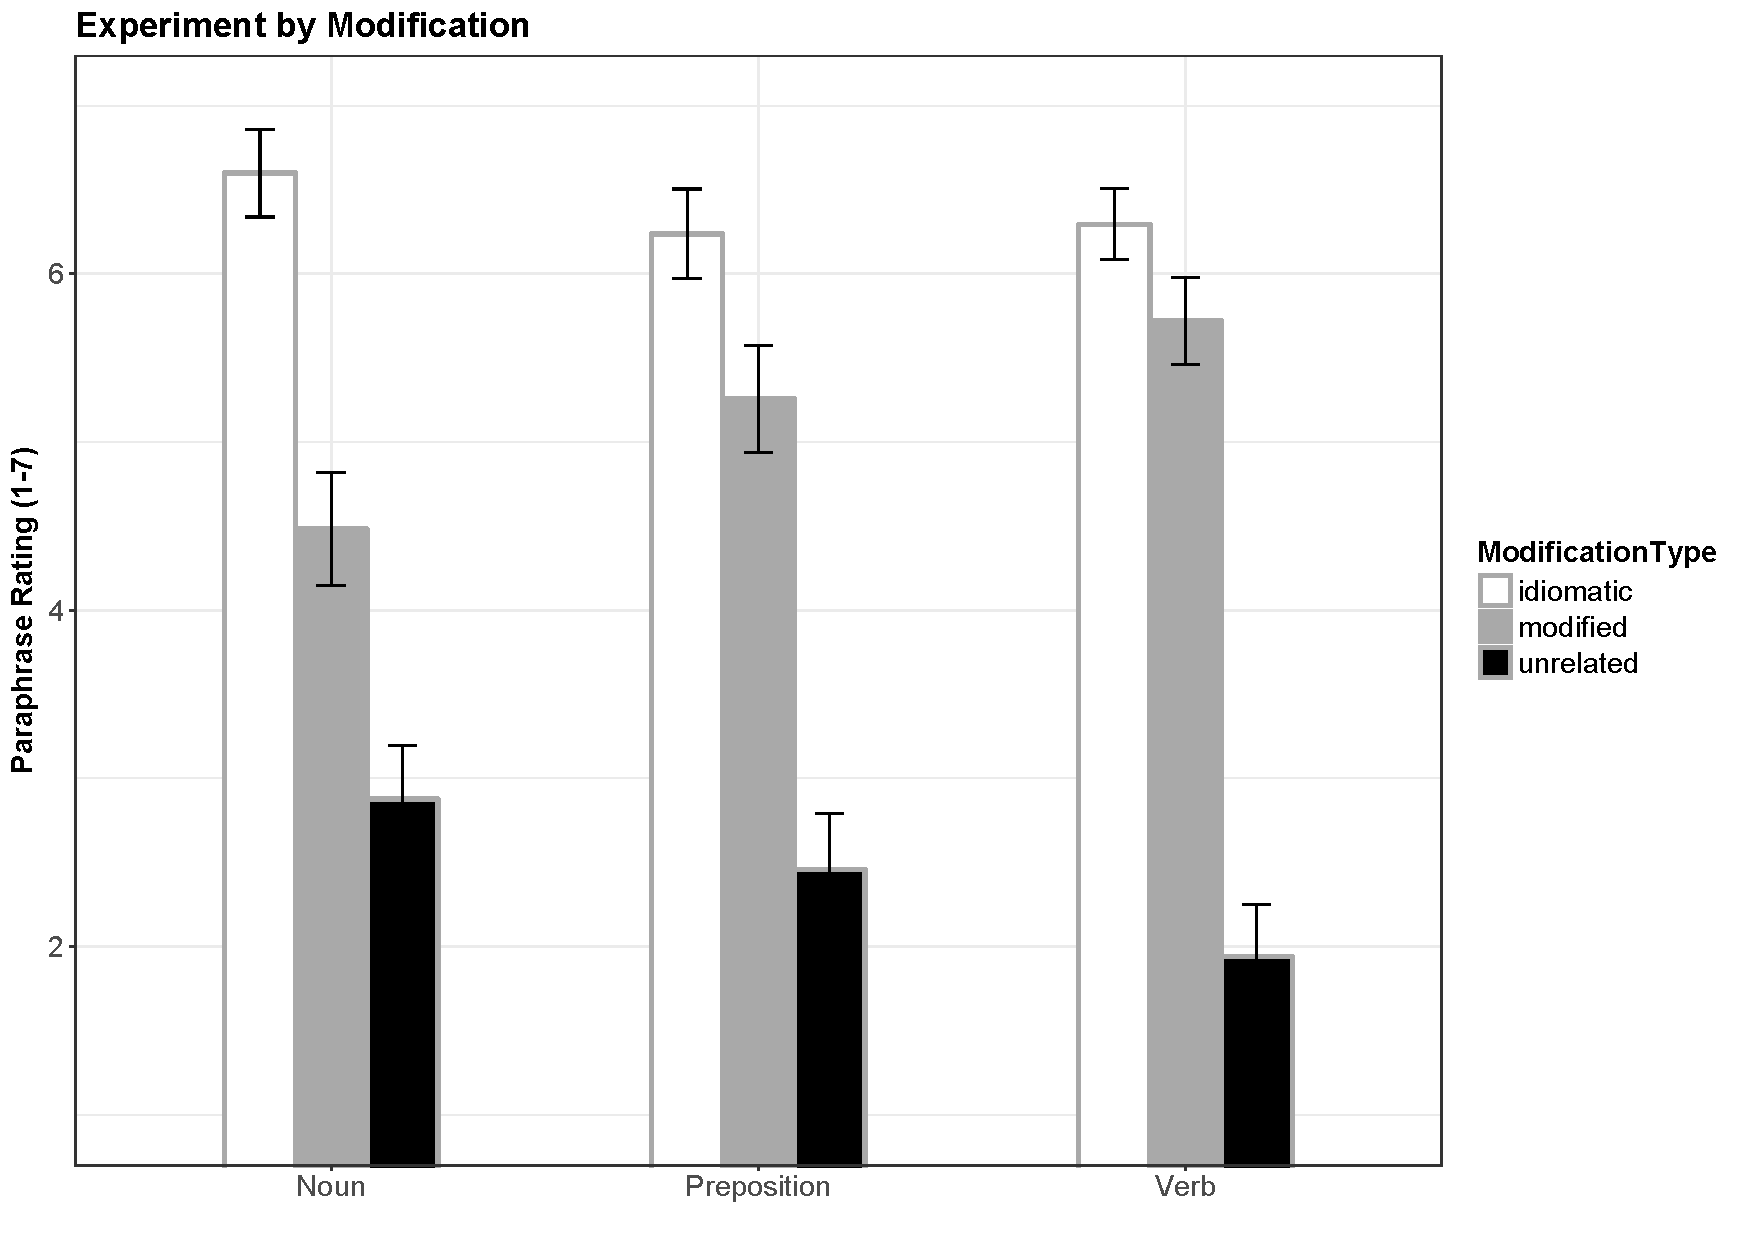
\includegraphics[width=\linewidth]{figures/smolka.pdf}
  \caption{Paraphrase ratings on a scale from 1--7 for idiomatic sentences holding idiomatic, modified, or unrelated constituents. Noun constituents were manipulated in Experiment 1 (left panel), prepositions in Experiment 3 (mid panel), and verb constituents in Experiment 2 (right panel). Y-bars indicate standard errors of the mean.}
  \label{fig:chart}
\end{figure}



\section{Experiment 2}

\subsection{Method}

\subsubsection{Participants}
Fifty-eight university students who had not participated in the previous experiment participated in the experiment for course credit or payment. All were native speakers of German. 

\subsubsection{Materials}
Thirty-three idiomatic phrases were selected for the sentence paraphrase test according to the same principles as in Experiment 1: They were fully idiomatic phrases as defined in Experiment 1 and were selected from the sentence pool described in Experiment 1. To ensure that their figurative meaning was the dominant reading, all had high sentence completion rates, that is, they were completed with verbs that produced the figurative meaning in 91\% of the cases (range 52\% to 100\%).

Each idiomatic sentence, such as \textit{Sie hat nach den Sternen gegriffen} (F: `She reached for the stars'), was cast in three versions, holding either (a) the canonical idiomatic verb (I), such as \textit{gegriffen} (‘reached’), (b) an associated verb (A), such as \textit{gelangt} (‘grasped’), or (c) an unrelated verb (U), such as \textit{gefragt} (‘asked’). In 26 of the 33 unrelated verbs, also the noun constituent that precedes the verb was modified to create a meaningful sentence, such as \textit{Sie hat nach den Sternzeichen gefragt} (L: `She asked for the zodiacs'). See Tables~\ref{tab:tripletsNouns}--\ref{tab:tripletsPrepositions} for examples of idiomatic sentences and their verb modifications.  \tabref{tab:exp2} provides the stimulus characteristics of the idiomatic sentences and the corresponding modifications.

\begin{table}
\caption{Idiomatic sentences and stimulus characteristics of the idiomatic, modified, and unrelated verb constituents in Experiment 2. \textit{Notes:} N = number of items, Lemma = mean lemma frequency per one million, taken from CELEX \citep{baayen:1993}, Closure = mean sentence completion in \%.\label{tab:exp2}}
\resizebox{\textwidth}{!}{\begin{tabular}{ccSSS}
\lsptoprule
 &  & \multicolumn{3}{c}{Type of noun}\\\cmidrule(lr){3-5}
& {Idiomatic phrase} & {Idiomatic} & {Modified} & {Unrelated} \\ \midrule
{Example} &  \textit{Sie hat nach den Sternen gegriffen} &  \textit{gegriffen} &  \textit{gelangt} & \textit{gefragt}\\ 
(translation) & (L: ‘She reached for the stars’) & {(‘reached')} & {(‘grasped')} &  {(‘asked')}\\
{N} &  & 33 & 33 & 33 \\ 
{Lemma} &  & 135 & 69 & 440 \\ 
{Surface} &  & 18.5 & 7 & 24.5 \\ 
{Association} &  & {--} & 5.3 & {--} \\ 
{Closure} &  & 90.9 & 0.46 & {--} \\ 
\lspbottomrule
\end{tabular}}
\end{table}

\subsubsubsection{Verb association test} 
Two verb associations (e.g. \textit{fassen} ‘grip’ and \textit{langen} ‘grasp’) were selected for each of the idiomatic verbs that should be modified (e.g. \textit{greifen} ‘reach’). It was taken care of that the verb associations were unrelated with the figurative phrasal meaning and that they generated a meaningful sentence. To avoid episodic effects, the same verb occurred only once in the whole experiment. 

The strength of the associations was assessed in a pre-test. The two associates of an idiomatic verb were allocated to two lists; in both lists, the idiomatic verb was paired with an associated and an unrelated verb.  For example, in List 1, the idiomatic verb \textit{greifen} (‘reach’) was presented with the association \textit{fassen} (‘grip’) and the unrelated verb \textit{kleben} (‘stick’); in List 2, \textit{greifen} (‘reach’) was presented with \textit{langen} (‘grasp’) and \textit{kleben} (‘stick’). Each list tested 112 verb pairs. 

Thirty participants (who did not participate in the paraphrase experiment) rated on a scale from 1 (not at all) to 7 (strongly) how strongly the meanings of the two verbs (e.g. \textit{greifen – langen}) are related. Verb associations were selected as associations of the original idiomatic verb, if they received high ratings (mean rating 5.8), and if their lemma and surface frequencies (taken from CELEX, see \citep{baayen:1993} were well matched with those of the idiomatic verb. 

\subsubsubsection{Paraphrases and fillers} The same procedure as in Experiment 1 was used to construct the paraphrases for each idiomatic phrase (see also Tables~\ref{tab:tripletsNouns}--\ref{tab:tripletsPrepositions}). In addition to the 33 idiomatic sentences, 22 literal sentences with the same sentence structure were used as fillers and were paired with unrelated paraphrases. 

\subsubsection{Procedure}

Participants were randomly assigned to a list. Paraphrase tests were distributed via email. Participants rated on a scale from 1 to 7 how strongly the two sentences reflected each other’s meanings. The instructions included two examples, one sentence pair with high meaning relatedness, the other sentence pair with low meaning relatedness. 
As in Experiment 1, three lists were constructed in such a way that each included one of the sentence triplets of an idiomatic phrase, either with the idiomatic (I), associated (A), or unrelated (U) verb. Each of the three sentence triplets was paired with the same paraphrase of the idiomatic sentence (see Tables~\ref{tab:tripletsNouns}--\ref{tab:tripletsPrepositions} for examples). The same 22 filler sentence pairs were added to each list, so that, altogether, each list comprised of 55 sentence pairs. The number of fillers ensured that 60\% of the sentences in a list were not meaning related with their paraphrase. 

\subsection{Results}
We applied the same LMM analyses as described in Experiment 1. The best model fit included the fixed-effect factor Modification Type and is summarized in \tabref{tab:Table5}; the right panel of \figref{fig:chart} depicts the paraphrase ratings. As in Experiment 1, paraphrase ratings were the highest to idiomatic phrases that held the canonical idiomatic verb (mean = 6.54, SD = 1.46), lower to phrases in which the canonical verb was modified by a closely associated verb (mean = 5.96, SD = 1.80), and the lowest to phrases with unrelated verbs (mean = 2.18, SD = 2.16). 

\begin{table}
\caption{Fixed effects of the predictors in the linear mixed-effect model for the paraphrase ratings in Experiment 2. \textit{Notes:} significance code: *** < 0.0001, ** < 0.01.\label{tab:Table5}}
\resizebox{\textwidth}{!}{\begin{tabular}{lS[table-format=-1.3]S[table-format=1.4]S[table-format=2.2]SS[table-format=<1.2e2]l}
\lsptoprule
 & {Estimate} & {Std. Error} & {df} & {$t$-value} & {$p$} &  \\ \midrule
(Intercept: Idiomatic) & 6.538 & 0.1389 & 112.2 & 47.07 & <2.00e-16 & *** \\ 
Constituent (Modified) & -0.580 & 0.1852 & 93.61 & -3.13 & 0.00234 & ** \\ 
Constituent (Unrelated) & -4.373 & 0.1853 & 93.68 & -23.61 & <2.00e-16 & *** \\ 
\lspbottomrule
\end{tabular}}
\end{table}

\section{Experiment 3}
\subsection{Method}
\subsubsection{Participants}

Fifty university students, all native speakers of German, participated in the experiment for course credit or payment.

\subsubsection{Materials}
Thirty-three idiomatic phrases were selected for the sentence paraphrase test according to the same principles as in Experiment 1: They were fully idiomatic phrases and selected from the same sentence pool as described in Experiment~1.  To ensure that their figurative meaning was the dominant reading, all had high sentence completion rates, that is, they were completed with words that produced the figurative meaning in 90.2\% of the cases (range 52\% to 100\%).

Each idiomatic sentence, such as \textit{Sie hat immer nach den Sternen gegriffen} (F: `She always reached for the stars'), was cast in three versions, holding either (a) the canonical idiomatic preposition (I), such as \textit{nach} (‘after’), (b) a modified preposition (A), such as \textit{zu} (‘to’), or (c) an unrelated prepositional phrase that held the same preposition as the idiomatic phrase (U), such as \textit{nach den Bonbons} (‘for the sweets’). See Tables~\ref{tab:tripletsNouns}--\ref{tab:tripletsPrepositions} for examples of idiomatic sentences and their prepositional modifications. \tabref{tab:Table6} provides the stimulus characteristics of the idiomatic sentences and the corresponding modifications.

\begin{table}
\caption{Idiomatic sentences and stimulus characteristics of the idiomatic and modified preposition, and unrelated prepositional phrase in Experiment 3. \textit{Notes:} N = number of items, Lemma = mean lemma frequency per one million, taken from CELEX \citep{baayen:1993}, Closure = mean sentence completion in \%.\label{tab:Table6}}
\resizebox{\textwidth}{!}{\begin{tabular}{ccSSS}\lsptoprule
 & & \multicolumn{3}{c}{Type of Preposition} \\\cmidrule(lr){3-5}
 & {Idiomatic phrase} & {Idiomatic} & {Modified} & {Unrelated PP} \\\midrule
{Example} & \textit{Ich habe ihn ins Herz geschlossen}                  & \textit{ins}  & \textit{ans}   & \textit{ins Zimmer} \\ 
(translation) & \multicolumn{1}{p{5cm}}{(L: ‘I locked him into the heart'\newline\hspaceThis{(}F: ‘I am fond of him')} & {(‘into')} & {(‘at the')} & {(‘into the room')} \\
{N} &  & 33 & 33 & 33 \\ 
{Lemma} &  & 6.7 & 4.2 &  {--} \\ 
{Closure} &  & 90.2 & {--} & {--} \\ 
\lspbottomrule
\end{tabular}}
\end{table}

\subsubsubsection{Preposition substitution}
Since prepositions may take many different meanings, so that association tests are not applicable, two native speakers selected a preposition (e.g. \textit{zu} ‘to’) that best matched the meaning of the idiomatic preposition (e.g. \textit{nach} ‘after’). We made sure that the modified preposition fitted the sentence frame and generated a meaningful sentence. As unrelated control condition, we used the idiomatic preposition and combined it with an unrelated noun phrase. 

\subsubsubsection{Paraphrases and fillers}
The same procedure as in Experiment 1 was used to construct the paraphrases for each idiomatic phrase. In addition to the 33 idiomatic sentences, 22 literal sentences with the same sentence structure were used as fillers and were paired with unrelated paraphrases.

\subsubsection{Procedure}

Three lists were constructed in such a way that each included the idiomatic phrase with either the canonical idiomatic preposition (I), the modified preposition (A), or the unrelated prepositional phrase (U). Each of the three sentence triplets was paired with the same paraphrase of the idiomatic sentence (see Tables~\ref{tab:tripletsNouns}--\ref{tab:tripletsPrepositions} for examples). Twenty-two fillers in each list reduced the relatedness proportion (between the sentences of a sentence pair) in a list to 40\%. The rest of the procedure was the same as in the previous experiments. 

\subsection{Results}

We applied the same LMM analyses as described in Experiment 1. The best model fit included the fixed-effect factor Modification Type only and is summarized in \tabref{tab:Table7}; the mid panel of \figref{fig:chart} depicts the paraphrase ratings. As in the previous experiments, paraphrase ratings were highest to idiomatic phrases that held the canonical idiomatic preposition (mean = 6.26, SD = 1.85), lower to phrases with a modified preposition (mean = 5.29, SD = 2.21), and lowest to phrases with an unrelated prepositional phrase (mean = 2.46, SD = 2.3).

\begin{table}
\caption{Fixed effects of the predictors in the linear mixed-effect model for the paraphrase ratings in Experiment 3. \textit{Notes:} significance code: *** < 0.0001\label{tab:Table7}}
\resizebox{\textwidth}{!}{\begin{tabular}{lS[table-format=-1.3]S[table-format=1.4]S[table-format=2.2]S[table-format=-2.2]S[table-format=<1.2e2]l}
\lsptoprule
 & {Estimate} & {Std. Error} & {df} & {$t$-value} & {$p$} &  \\ \midrule
(Intercept: Idiomatic)  & 6.260             & 0.1768              & 133.04      & 35.42            & <2.00e-16 & *** \\ 
Constituent (Modified)  & -0.973            & 0.2099              & 96.36       & -4.63            & 1.13e-05  & *** \\ 
Constituent (Unrelated) & -3.797            & 0.2099              & 96.40       & -18.09           & <2.00e-16 & *** \\ 
\lspbottomrule
\end{tabular}}
\end{table}


\section{Post-hoc analysis of experiments 1--3}    

The results of all three experiments showed that idiomatic constituents may be modified by a close associate and still yield the figurative meaning. A visual inspection of \figref{fig:chart} suggests that modified verbs are better in yielding the figurative meaning than either nouns or prepositions. The following LMM analysis was conducted to test whether the word category of a constituent (noun, verb, preposition) affects whether its modification is considered as reflecting the figurative meaning better. 

We applied the same LMM analysis as in the previous experiments. As random effects, we had intercepts for participants and items (i.e. sentences). In addition to the previously used fixed effects -- Modification Type (idiomatic\slash associated\slash unrelated), the Sentence Closure of the idiomatic phrase, and the Frequency of the constituent (log-transformed and centered, absolute lemma frequencies from CELEX) -- we included the factor Experiment (corresponding to the tested constituent).  We applied a forward procedure for the model selection, and obtained the best model fit by comparing the Akaike Information Criterion (AIC) statistics between models. 

The best model fit included the fixed-effect factors Modification Type and Experiment, and an interaction between the two.  \tabref{tab:Table8} summarizes the effects. The results reflect the findings depicted in \figref{fig:chart}.  Overall speaking, as in each of the Experiments 1--3, paraphrase ratings were highest to idiomatic phrases that held the canonical constituent, lower to phrases in which the canonical constituent was modified by a closely associated constituent, and lowest to phrases with unrelated constituents. Across experiments notwithstanding, sentences with modified preposition or verb constituents received higher ratings and were thus perceived as better representing the figurative meaning than sentences with modified nouns. Further, sentences holding unrelated verbs received lower paraphrase ratings than sentences holding unrelated nouns, indicating that unrelated verbs are perceived as lowest in representing the figurative meaning. 

\begin{table}
\caption{Fixed effects of the predictors in the linear mixed-effect model for the paraphrase ratings combining Experiments 1--3. \textit{Notes:} significance code: *** < 0.0001, * < 0.05.\label{tab:Table8}}
\resizebox{\textwidth}{!}{\begin{tabular}{p{4.5cm}SSSS[table-format=<1.2e1]l}\lsptoprule
& {Estimate} & {Std. Error} & {$t$-value} & {$p$} &  \\ \midrule
(Intercept: Idiomatic, Noun) & 6.245 & 0.159 & 39.18 & <2.00e-16 & *** \\ 
Constituent (Modified)       & -2.115 & 0.193 & -10.96 & <2.00e-16 & *** \\ 
Constituent (Unrelated)      & -3.895 & 0.183 & -21.25 & <2.00e-16 & *** \\ 
Experiment (Preposition)     & 0.033 & 0.161 & 0.20 & 0.8396 &  \\ 
Experiment (Verb)            & 0.381 & 0.161 & 2.38 & 0.0182 & * \\ 
Constituent (Modified) \newline\hbox{}\hspace{2em} x Experiment (Prep.)  & 1.122 & 0.233 & 4.82 & 2.09e-06 & *** \\
Constituent (Unrelated)\newline\hbox{}\hspace{2em} x Experiment (Prep.) & 0.248 & 0.177 & 1.40 & 0.1613 &  \\ 
Constituent (Modified) \newline\hbox{}\hspace{2em} x Experiment (Verb)   & 1.454 & 0.233 & 6.24 & 1.18e-09 & *** \\
Constituent (Unrelated)\newline\hbox{}\hspace{2em} x Experiment (Verb)  & -0.443 & 0.214 & -2.07 & 0.0386 & * \\ 
\lspbottomrule
\end{tabular}}
\end{table}

\section{General discussion}
The present study investigated whether idioms are semantically fixed, as suggested by established linguistic and psycholinguistic models on the processing and production of idioms. We asked first, whether idiomatic constituents may be modified while retaining the figurative meaning, and second, whether some idiomatic constituents are more susceptible to modification than others in keeping the figurative meaning. 

Previous studies observed that idiomatic verb constituents activate their literal meaning while they contribute to the activation of the figurative meaning (e.g., \citealt{rabanus:2008}; \citealt{smolka:2007}). In the present study, we thus asked whether not only the constituent itself but also a close associate of the constituent (that activates a similar literal meaning) will contribute to the activation of the figurative meaning. We compared the processing of canonical idiomatic phrases like \textit{Sie hat immer nach den Sternen gegriffen} (L: ‘She always reached for the stars’) with sentences in which one of the idiomatic constituents (i.e., the noun, verb, or preposition) was modified by a close semantic associate, as in \textit{Sie hat immer nach/zu den Sternen/Planeten gegriffen/gelangt} (L: ‘She always reached/grasped for/to the stars/planets’). The results of the paraphrase ratings indicated that the figurative meaning of the idiom is recognized even when a semantic associate replaces the canonical idiom constituent. That is, modified idiomatic constituents may contribute to the generation of the figurative meaning of the idiom. 

Our findings confirm the findings by \citet{geeraert:2017} that the figurative meaning is accepted when idiomatic noun constituents are modified by near synonyms or semantic associates (e.g. \textit{they went through the ceiling}).  We have extended the finding on noun constituents to other idiomatic constituents, such as the verb and the preposition, and have shown that they may be modified as well. Indeed, the modifications of all types of constituents (nouns, verbs, and prepositions) were rated as better reflecting the figurative meaning than unrelated constituents. 

We further asked whether a particular type of constituent (noun, verb, or preposition) more strongly preserves the figurative meaning than others.  Indeed, our results show that modified verbs are stronger than modified nouns or prepositions at activating the figurative meaning. This finding fits well with the assumption by \citet{hamblin:1999} that the meaning of the verb in idiomatic phrases may influence the meaning of the idiom. When a verb such as \textit{kick} in \textit{kick the bucket} was replaced by a verb that expressed the fast and sudden action, such as \textit{punt}, this substitution was rated as better preserving the meaning of the idiom than a verb that did not represent the inherent meaning of the verb, such as \textit{nudge}. Hamblin and Gibbs concluded that the verb-inherent action was transferred to the meaning of the whole idiomatic phrase.

In the following paragraphs, we are searching for a plausible reason why the modified verb more strongly activates the figurative meaning than a modified noun or preposition does: Since there are, to our knowledge, no studies that directly compare the processing of different idiomatic constituents (nouns, adjectives, verbs, prepositions) and how each contributes to the overall figurative meaning, we are allowing ourselves to speculate why verb constituents of idioms are differently processed than noun or prepositional constituents. 

The processing of modified verbs similar to canonical ones may have been further facilitated by the fact that in the present study verbs occupy the sentence-final position.  From a semantic perspective, the verb is thus partly processed even before it has been encountered.  Consider the German idiom \textit{Ich habe ihn sehr ins Herz geschlossen} (L: `I locked him into the heart'; F: `I am very fond of him'). The German preposition \textit{in(s)} governs both the dative case for locations (indicating the semantic feature [+static]) and the accusative case for directions (indicating the feature [\textendash static]; \citealt{gansel:1992}). Because the above example assigns an accusative, the semantic feature [\textendash static] of the participle \textit{geschlossen} (‘locked’) can be anticipated. Hence, certain semantic properties of the verb are processed before it is realized.

Also from a syntactic perspective, the verb is partially processed even before it has been encountered. According to valency theory (e.g., \citealt{tesniere:1959}), the verb controls the syntactically obligatory complements.\footnote{With respect to literal language, the verb’s valency (i.e. the number of complements it requires) was shown to affect both language production (e.g., \citealt{thompson:1997}) and language comprehension \citep{shapiro:1987}. However, the verb’s valency did not affect the processing of figurative language: Idiomatic sentences holding transitive verbs (that require one obligatory complement) and idiomatic sentences holding ditransitive verbs (that require two obligatory complements) were processed equally fast \citep{dorrestars}.} These complements, in turn, are dependent on the subcategorization properties of the verb and are predictable as soon as the verb has been processed. In our sentences, where the verb occupies the sentence-final position, the direction of predictability is reversed: The number and type of complements that occur in the sentence constrain the choice of possible verbs in the last position, so that the verb is partially processed even before it has been encountered.


Moreover, the high cloze probabilities of sentences in the present experiments indicate that participants expect the meaning of a specific verb in sentence-final position. Hence, the meaning of the idiomatic verb constituent was activated before it was encountered, so that the modified verb, which activates a similar literal meaning, is stronger in activating the figurative meaning than other (noun or preposition) constituents that are not as expected. 


To summarize, if we assume that (a) the verb-inherent action is transferred to the figurative meaning of the idiom (see \citealt{hamblin:1999}), and (b) the literal meaning of the verb remains activated even after the figurative meaning of the idioms has been recognized (see \citealt{rabanus:2008}; \citealt{smolka:2007}), (c) the syntactic and semantic properties of the verb in the sentence-final position are partly processed before it is encountered, the possibility that a close associate of the verb (that activates a literal meaning similar to that of the canonical verb) will trigger the figurative meaning of the idiom.  


Overall, the present findings provide evidence against any type of model on idiom comprehension or production that assumes some kind of fixed lexical entry of the idiomatic constituents that generate the figurative meaning, including fixed idiom words \citep{bobrow:1973}. The present findings also disagree with hybrid models that assume a unitary or fixed representation to capture the idiosyncratic meaning of an idiom, such as the fixed word configuration in form of an idiom key (e.g., \citealt{cacciari:1988}), fixed superlemmas (e.g., \citealt{sprenger:2006}), or fixed lexical concept nodes (e.g., \citealt{cutting:1997}). For example, according to the configuration hypothesis \citep{cacciari:1988}, the Italian sentence \textit{Dopo l’ottima prestazione, il tennista era al settimo cielo} (F: `After the excellent performance, the tennis player was in seventh heaven') is processed literally until the specific word configuration \textit{to be in seventh heaven} is recognized to form the figurative meaning. As soon as the figurative meaning is hit, the literal meaning activation is dropped and no longer active. Accordingly, the presentation of the noun constituent \textit{cielo} (‘heaven’) did not activate its literal association \textit{stelle} (‘stars’). Because the configuration hypothesis assumes that only the very specific word configuration -- the idiom key -- renders the figurative meaning, a sentence with a modified word configuration such as \textit{The tennis player was in seventh sky} should not be able to activate the figurative meaning. 


A similar assumption underlies the concept of the superlemma \citep{sprenger:2006}: A superlemma such as [hit-the-road] specifies the single constituents of the idiom (i.e., \textit{hit, the, road}) as well as their syntactic features and functions. It engages morphosyntactic constraints on the idiomatic configuration to discriminate idiomatic from literal word configurations \citep{sprenger:2006}. Hence, the morphosyntactic constraints of the superlemma [hit-the-road] could not apply to modified constituents such as \textit{hit the street} or \textit{strike the road} and would not retrieve a figurative meaning. 


Overall, the present findings provide evidence against any noncompositional lexical representation of the figurative meaning of idioms. By contrast, the present findings fit well with the recent study on idiom variation referred to above \citep{geeraert:2017}. Baayen and colleagues modelled their findings in a naïve discrimination learning (NDL) account \citep{baayen:2013,baayen:2011,baayen:2016} that entails sublexical orthographic units such as letter trigrams that are mapped onto meaning units in form of so-called lexomes. The lexome of an idiom corresponds to a pointer to its semantic vector like \textit{to die} that is activated by the different letter triplets that the idiom holds. Importantly, the many different inputs may activate the same lexome, so that \textit{to die, pass away,} and \textit{kick the bucket} will all activate the same lexome \textit{die}. This may explain why idioms with modifications may be acceptable to some degree. However, given that the NDL account does not recognize abstract linguistic categories, such as nouns, verbs, or prepositions, it is unclear how it could account for the finding that the modification of verbs is more effective than nouns or prepositions at activating the figurative meaning. 

Finally, the present findings fit well with the stem-based account \citep{gunther:2018,rabanus:2008,smolka:2017,smolka:2007,smolka:2014,smolka:2015,smolka:2018}, which is a unitary system for the processing of literal and figurative language: Stems of multiword expressions -- ranging from complex verbs and compounds to idioms -- activate the literal meanings of the stems, and together the stems co-activate their joint figurative meaning.\footnote{Even though the literal meaning of a constituent is assumed to be activated, figurative meanings are not second-level interpretations that necessitate complete literal interpretations of the utterances on the first level. Rather, figurative interpretations do not block the activation of literal associations (see \citealt{gibbs:2002}).} This holds for the meanings of semantically transparent and opaque complex verbs (e.g., \textit{understand}) and compounds (e.g., \textit{hogwash}) just as for the opaque meaning of idioms (\textit{kick the bucket}). Because the literal meaning of a constituent is activated alongside the figurative meaning of the multiword expression, semantically associated words that activate a similar meaning as well as that of the idiomatic constituent will contribute to the figurative meaning assembly. 

\section{Conclusion}
The present findings indicate that lexical representations of idioms are not as semantically fixed as has been assumed so far: Modified constituents that activate meanings similar to those of the canonical constituents will co-activate the figurative meaning of the idiom together with the other idiomatic constituents. Modified verb constituents more strongly activate the figurative meaning than modified noun or prepositions do. Future studies will be necessary to examine how many idiomatic constituents may be modified at once (e.g., \textit{grasp at the planets}) while keeping the figurative meaning of the idiom (e.g., \textit{reach for the stars}).

\section*{Acknowledgements}
This study was supported by Grant FP561/11 by the Volkswagen Foundation to Eva Smolka. Experiment 1 was part of \ia{Baumann, Sarah@Baumann, Sarah}Sarah Baumann's M.A. thesis, we thank her for conducting the experiments.

% % % % \let\cleardoublepage\clearpage % <- Some people just want to watch the world burn.

{\sloppy\printbibliography[heading=subbibliography]}
\end{document}
